\subsection{Systemarchitektur}\label{sec:system_rough}

Aus den zu lösenden Anwendungsfällen und Problemen sowie den verschiedenen bekannten Lösungsansätzen lässt sich die in Abbildung \ref{fig:system_rough} skizzierte Systemarchitektur ableiten. Die darin gezeigte Struktur und die aufgezeigten Datenaustausch-Pfade beschreiben dabei den Datenfluss zwischen den Komponenten\footnote{Auf die Verwendung eines exakteren, formalen Datenflussdiagrammes wurde aus Gründen der Übersichtlichkeit verzichtet.}. Sie baut sich aus den folgenden Bestandteilen auf:

\begin{itemize}
\item Der \textbf{Nutzer} steht an Beginn und Ende der Interaktionswege. Durch seine Interaktion mit der Webseite wird ein entsprechendes Profil erstellt, welches es ermöglichen soll Suchergebnisse und Webseiteninhalte  zu Personalisieren (vgl. Abschnitt \label{sec:userstories})
\item Die \textbf{Webseite} mit der eingebetteten \textbf{Suche} stellt das Interaktionsmedium für den Nutzer dar. Zudem sollen mit Hilfe der eingebetteten \glslink{Tracking}{Tracking-Mittel} die Interaktionen des Nutzers aufgezeichnet werden.
\item Der \textbf{Tracker} dient der Aufzeichnung der Interaktionen des Nutzers mit der Webseite. Er stellt sicher, dass die aufgezeichneten Daten verlustfrei in den Datenspeicher übertragen werden. Er muss den in Abschnitt \ref{sec:performancereq} beschriebenen Leistungsanforderungen bei der Datenerhebung genügen.
\item Die \textbf{Datenhaltung} erfolgt auf den in Abschnitt \ref{sec:hfs} beschriebenen Grundlagen. Sie soll sicherstellen, dass Daten zwischen mehreren  Servern effizient verteilt werden können und ermöglich die Ausführung von \textit{MapReduce}-Programmen (vgl. Abschnitt \ref{sec:mapred}) für diese Daten.

\begin{figure}[H]
  \centering
    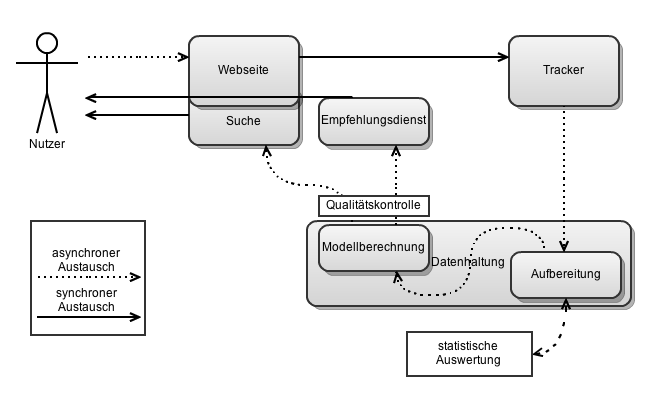
\includegraphics[width=\textwidth]{Abbildungen/Systemmodell.png}
    \caption[Systenarchitektur]{\footnotesize Systemarchitektur-Entwurf der alle notwendigen Komponenten und den Interaktionsfluss umreißt}
    \label{fig:system_rough}
\end{figure}

\item Die \textbf{Datenaufbereitung} analysiert die vom Tracker geschriebenen Interaktionsprotokolle aller Nutzer und führt notwendige Vorverarbeitungsschritte durch. Das Ergebnis der Vorverarbeitung sind zum einen kompakte Nutzerprofile die der in Abschnitt \ref{sec:cf_overview} beschriebenen \textit{User-Item} Matrix entsprechen. Ein weiteres Ergebnis welches sich bei der Datenaufbereitung gewinnen lässt, sind verschiedene Maße zur Qualitätskontrolle bzw. zur statistischen Auswertung (vgl. Abschnitt \ref{sec:measure_c}).
\item Bei der \textbf{Modellberechnung} werden mit Hilfe der in Abschnitt \ref{sec:neighborhoods} und \ref{sec:svd} beschriebenen Methoden alle notwendigen Berechnungen zur Bildung der Ähnlichkeitsmodelle bzw. zur Matrixfaktorisierung durchgeführt. Ebenso wie die Datenaufbereitung erfolgt sie verteilt auf den Datenhaltungs-Servern, zum Beispiel durch die Ausführung vom \textit{MapReduce}-Programmen. Vor der anschließenden Nutzung, müssen sie einer Qualitätskontrolle unterzogen werden. Dies kann durch die Überwachung der in Abschnitt \ref{sec:measures} beschriebenen Maße erfolgen.
\item Der \textbf{Empfehlungsdienst} nutzt das Ergebnis der Modellberechnung um Empfehlungen für die Anfragen einzelner Nutzer zu generieren. Durch die direkte Nutzung des Empfehlungsdienstes wird die Umsetzung der Anwendungsfälle zu kontextbasierten Empfehlungen, Komplementär-Suchen und Cross-Selling ermöglicht.  Er muss den in Abschnitt \ref{sec:performancereq} beschrieben Leistungsanforderungen zur Personalisierung genügen.
\item Die Ergebnisse der \textbf{Suche} werden durch die Ausgabe des Empfehlungsdienstes den Präferenzen des Nutzers entsprechend priorisiert. Mit dem in Abschnitt \ref{sec:myrecommend} beschriebenen Ansatz, ist es zudem möglich, die Ergebnisse der Modellberechnung der Matrixfaktorisierung direkt in der Suche zu nutzen und damit bei der Personalisierung auf einen separaten Empfehlungsdienst zu verzichten. Wie der Empfehlungsdienst muss auch die Suche den in Abschnitt \ref{sec:performancereq} beschrieben Leistungsanforderungen zur Personalisierung genügen.
\end{itemize}

Wie in der Abbildung aufgezeigt ist, soll der Datenaustausch zwischen einigen Komponenten asynchron verlaufen. Dies entspricht den in Abschnitt \ref{sec:scale2} beschriebenen Lösungsstrategien zur Skalierbarkeit. Es ermöglicht ohne zusätzliche Anpassung der Kommunikationswege, dass jede der Komponenten bei Bedarf auch auf mehrere Server verteilt werden kann.

Da die Verarbeitung der Daten und die Erstellung neuer Modellberechnungen im produktiven Betrieb möglichst regelmäßig durchgeführt werden muss, wird zudem ein zentraler Dienst zur Steuerung bzw. Überwachung des Ablaufs benötigt. Da dieser keinen besonderen Anforderungen entsprechen muss und die Bandbreite der möglichen Lösungswege den Rahmen der Arbeit sprengen würde, kann in der weiteren Betrachtung stets von einfachen zeitgesteuerten Prozessen ausgegangen werden. \todo{Ggf Zookeeper oder MQ Konzeptelink ergänzen / Kapitel verlinken}
